%% chapter 7, LCS03, convergence analysis
%\input{header}
%\usepackage{verbatim}
%\usepackage[latin1]{inputenc}
%\usepackage{tikz}
\usetikzlibrary{calc}
\usetikzlibrary{shapes,arrows}
%\usepackage{enumerate}
%% \newcommand{\midarrow}[1]{\stackrel{#1}{\to}}
%
%% \newcommand{\Real}{\mathbb R}
%% \newtheorem{assumption}{Assumption}
%\begin{document}
%
%
%% First page number
%\setcounter{page}{1}
%% PREVIOUS section number
%\setcounter{section}{6}
%% PREVIOUS subsection number
%\setcounter{subsection}{0}
%
%% ***********************************************************************
%\textsc{Reinforcement Learning and Dynamic Programming \hfill Spring 2014$\;$ \\
%Lecture Notes \hfill Shie Mannor and Nahum Shimkin \\
%\hfill Scribed by Michal Zarrouk}
%\vspace{-18pt}
%\par
%\hrulefill
%% ***********************************************************************
%
%% {\large
%
%

\newcommand{\weights}{\texttt{w}}
\newcommand{\ftrs}{\phi}
\newcommand{\FtrMtx}{\Phi}
% \newcommand{\state}{\texttt{s}}
% \newcommand{\policy}{\pi}


%\section{Approximate Dynamic Programming}
Recall Bellman's dynamic programming equation
$$V(s) = \max_{a \in A} \left\{R(s,a) + \gamma \sum_{s' \in S} p(s'|s,a)V(s')\right\},$$
or in operator form, $\underline{V}=T\underline{V}$, where $T$ is the Bellman operator.

Dynamic programming requires knowing the model and is only feasible for small problems.
In large scale problems, we face the \textbf{3 curses of dimensionality}:

\begin{enumerate}
\item $S$ may be large, such that even writing down the policy is difficult. Moreover, $S$ may be continuous, for example in robotics applications.
\item $A$ may be large. Example: resource allocation, where we have several projects and need to assign different resources to each project.
% Note: give details
\item $p(s'|s,a)$ may be complicated: computing $p(s'|s,a)$ requires summing over many random events. Example: resource allocation.
\end{enumerate}

\section{Approximation approaches}
There are 4 approaches to handle the curses of dimensionality:
\begin{enumerate}
\item \textbf{Myopic}: When $p(s'|s,a)$ is approximately uniform across $a$, we may ignore the state transition dynamics and simply use $a^\pi(s)\approx \underset{a \in A}{\operatorname{argmax}} \{R(s,a)\}$. If $R(s,a)$ is not known exactly -- replace it with an estimate.

\item \textbf{Lookahead policies}: Rolling horizon/model-predictive control.\\
Simulate a horizon of $T$ steps, and use
$$a^\pi(s_t) = \underset{\pi' \in \Pi}{\operatorname{argmax}}\  \mathbb{E}^{\pi'} \left[\left.\sum_{t'=t}^{t+T} R(s_{t'},\pi'(s_{t'}))\right|s_t\right]$$

\item \textbf{Policy function approximation}\\
Assume policy is of some parametric function form $\pi = \pi(\weights), \ \ \weights \in \mathtt{W}$, and optimize over function parameters.\\
\begin{example}[Inventory management]
Consider an inventory management problem, in which the state is the inventory level $s_t$, the demand is $d_t$ and the action is the replenishment level $a_t$. The dynamics are given by:
$$s_{t+1} = [s_t + a_t-d_t]^+.$$
The immediate reward is:
$$R_t = R \min\{d_t,s_t+a_t\} - c_a a_t -C[s_t + a_t-d_t]^+,$$
where $R$ is the profit in satisfying the demand, $c_a$ is the ordering cost, and $C$ is the cost of not satisfying a demand.

One possible replenishment policy is:
$$a^\pi(s_t|\weights) = \begin{cases} 0 & s_t > q\\Q-s_t & s_t \le q \end{cases}, \ \ \ \weights=(q,Q).$$
A different possibility is the \emph{softmax} policy, given by
$$p(s,a) = \frac{e^{-\weights\alpha(s,a)}}{\sum_{a'} e^{-\weights\alpha(s,a')}}, \ \ \mathrm{where}\ \ \alpha=R(s,a)\ \ \mathrm{or} \ \ \alpha=Q(s,a).$$
\end{example}

\item \textbf{Value function approximation}\\
Assume $V(s)\approx \bar{V}(s,\weights)$ where $\bar{V}$ is some approximation function, and optimize over the parameters $\weights$.\\
The most standard model is a linear combination of some $k$ features (which are not necessarily linear):
$$\bar{V}(s|\weights) = \sum_{j=1}^k \weights_j \ftrs_j(s),$$
where $\weights_j$ are the model parameters and $\ftrs_j$ are the model's \emph{features} (a.k.a. basis functions).\\
Given $\bar{V}$, we can derive a policy by choosing the \emph{greedy} action with respect to $\bar{V}$ (corresponding to a lookahead of 1 time step). If a model or a simulator is also available, we can also use a longer lookahead.\\
\\
Example: a chess game with $K$-step lookahead\\
\tikzstyle{block} = [rectangle, draw,
    text width=7em, text centered, rounded corners, minimum height=4em]
\tikzstyle{blocks} = [rectangle, draw,
    text width=4em, text centered, rounded corners, minimum height=4em]
\tikzstyle{lblock} = [rectangle, draw,
    text width=17em, text centered, rounded corners, minimum height=4em]
\tikzstyle{line} = [draw, -latex']
\begin{tikzpicture}[node distance = 1cm, auto]
    % Place nodes
%    \node [blocks] (a) {Chess game model};
    \node [block] (b) {Feature extraction\\$\ftrs_1(s),...,\ftrs_k(s)$};
    \node [block, right of = b, node distance=1.3in] (c) {Compute value\\function weights\\$\weights_1,...,\weights_k$};
    \node [block, right of = c, node distance=1.3in] (d) {$\bar{V}(s)=f(s,\weights)$};
    \node [lblock, right of = d, node distance=2.1in] (e) {\small$\pi(s_t) = \underset{\pi' \in \Pi}{\operatorname{argmax}}\  \mathbb{E}^{\pi'} \left[\sum_{t'=t}^{t+K-1} R(s_{t'}) + \bar{V}(s_{t+K}))\right]$};
    % Draw edges
%    \path [line] (a) -- (b);
    \path [line] (b) -- (c);
    \path [line] (c) -- (d);
    \path [line] (d) -- (e);
\end{tikzpicture}

\paragraph{Issues:}
\begin{enumerate}
\item Choosing the parametric class $\ftrs$ (architecture): e.g., Radial Basis Functions (RBFs) or kernels. The difficulty is that the value function structure may be hard to know in advance.
\item Tuning the weights $\weights$ (learning): here we focus on simulation.\\
In the linear architecture, we can write
$$\tilde{V}(s;\weights)=\ftrs(s)^\top \weights$$
(replacing $\weights$ with $r$ for the parameters), or in matrix-vector form,
$$\tilde{ {V}}( {\weights}) =  { {\FtrMtx}} { \weights}$$
Therefore tuning the parameters $ {\weights}$ reduces to approximating $ {V} \in \mathbb{R}^{|S|}$ on $\mathcal{S}=\{  { {\FtrMtx}} {\weights}:  {\weights} \in \mathbb{R}^k\} \subseteq  \mathbb{R}^{|S|} $.

\end{enumerate}

\end{enumerate}

\section{Lookahead Policies}

We will discuss several variants of lookahead policies. We focus on systems with a discrete, and `small enough' action space, but a large, possibly infinite state space.

The main idea in lookahead policies is that when we are at some state $s$, we will only search `around' the state $s$ for the next action $\pi(s)$. After we play the action, we observe the next state, and repeat the search.
Thus, we do not need to consider the whole state space in advance, but only consider regions in state space which we actually visit.
In the control literature, this idea is often called Model Predictive Control (MPC).

\subsection{Deterministic Systems: Tree Search}
The simplest example of a lookahead policy is tree search in a deterministic system.

Given $s$, and a (deterministic) simulator of the system, we can simulate the next state for every possible action, building a tree of possible trajectories of the system, starting from $s$, and continuing to some depth $k$. 
We then choose an action by:
$$\pi(s) = \underset{\pi' \in \Pi}{\operatorname{argmax}}\  \left[\left.\sum_{t=0}^{k} \gamma^t r(s_{t},{\pi'}(s_{t})) \right| s_0 = s\right],$$
Which can be solved using dynamic programming.

In this approach, the computation in each step requires $O(|A|^{k})$ calls to the simulator for building the tree, and $O(k|A|^{k})$ computations for searching the tree. Note that \emph{there is no dependence on $|S|$}. The depth $k$ should be chosen `deep enough' to results in meaningful actions. For example, in a discounted setting, recall that the $k$-horizon value function satisfies 
$\|V^k(s)-V^*(s)\|_\infty \leq \gamma^k\left( \frac{R_{max}}{1-\gamma}\right),$ which can be used to set $k$.

\subsection{Stochastic Systems: Sparse Sampling}
When the system is stochastic, we cannot simply build a tree of possible future trajectories. If we sample next states from our simulator, we can build a \emph{sampled} version of a search tree. Here, for each state $s$ and action $a$ in the tree, we will sample $C$ next states $s'_1,\dots,s'_C$. Then, the backup at $s,a$ will be $Q(s,a) = \frac{1}{C}\sum_{i=1}^C r(s,a) + \gamma \max_{a'} Q(s'_i,a')$.
That is, we replaced the expectation in the Bellman update with an empirical average. Since the average concentrates around the mean (e.g., by Hoeffding inequality), it is expected that the empirical averages will closely represent their expectations.

The following result is shown in \cite{kearns2002sparse}. The constants $k$ and $C$ can be set such that with a per-state running time of $(\frac{|A|}{\epsilon (1-\gamma)})^{O\left(\frac{1}{1-\gamma}\log \frac{1}{\epsilon (1-\gamma)}\right)}$, the obtained policy is $\epsilon-$optimal, i.e., $\|V^k(s)-V^*(s)\|_\infty \leq \epsilon$. Note again that there is no dependence on $|S|$.

\subsection{Monte Carlo Tree Search}
While the sparse sampling above does not depend on $|S|$, the exponential dependence on the horizon and number of actions makes it impractical for many cases. The insight in Monte-Carlo Tree Search (MCTS) is that investing the same simulation efforts for all possible future actions is wasteful, and we should instead focus our search efforts on the \emph{most promising} future outcomes.

The first idea in MCTS is to replace the stage-wise tree building approach with a rollout-based approach, as shown in Figure \ref{fig:mcts}. Here, we roll out complete trajectories of depth $k$, and build the tree progressively from these rollouts. The method \textbf{Evaluate(state)} is used to evaluate the last state in the rollout. This could be the reward of the state, or an estimated value function (as in the chess example above). Another approach, which has become common in games such as Go and Chess, is to simulate a game starting from state $s$ with a predetermined policy, until termination, and evaluate the state by the empirical return along the simulation trajectory.
The method \textbf{UpdateValue} is used to build the tree. It maintains both the sum of returns from a state action pair $Q_{sum}(s,a)$ (summing over all trajectories that visited this state), and the number of visits to the state and state-action pair, $N_s$ and $N_{sa}$. The value of a state-action pair is the average $\frac{Q_{sum}(s,a)}{N_{sa}}$. To understand why this approach could be beneficial, consider a state that is visited multiple times. Thus, after several visits, we have some information about which actions are more promising, and could use that to bias the rollout policy to focus on promising trajectories. We need to make sure, however, that we also \emph{explore} often enough, so that we do not miss important actions by incorrect $Q$ estimates in the beginning.
The key to an efficient MCTS algorithm, therefore, is in the \textbf{selectAction} method, which should balance exploration and exploitation.

\begin{figure}[h]
    \centering
    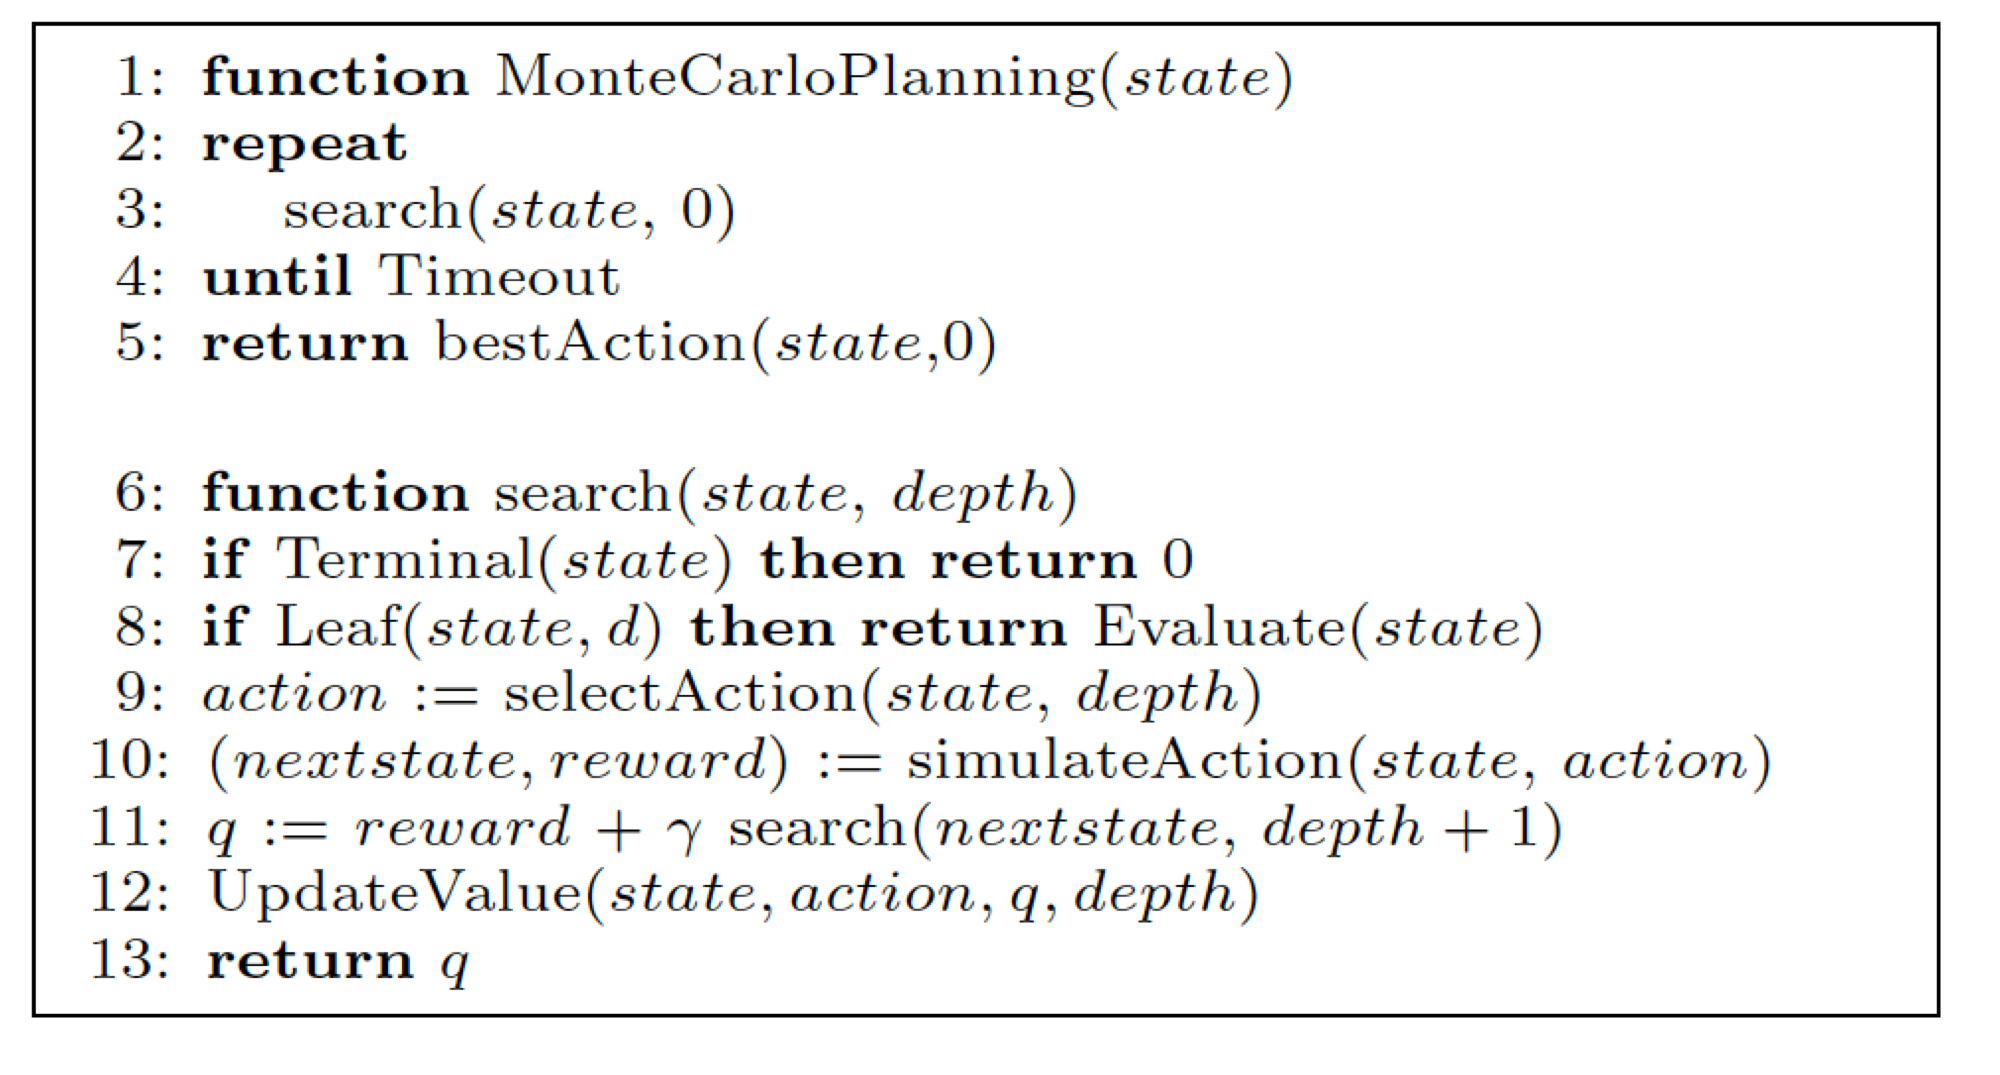
\includegraphics[width=0.8\textwidth]{figures/uct.png}
    \caption{Generic Monte-Carlo Planning Algorithm (from\cite{kocsis2006bandit})}
    \label{fig:mcts}
\end{figure}

The UCT algorithm of Kocsis and Szepesv´ari~\cite{kocsis2006bandit} selects actions that maximize $Q(s,a) + UCT(s,a)$, where the \emph{upper confidence bound} is given by: 
$$
UCT(s,a) = C \sqrt{\frac{\log N_s}{N_{sa}}},
$$
where $C$ is some constant. Intuitively, $UCT$ prefers actions that are either promising (high $Q$) or under-explored (low $N_{sa}$). Later in the course we will show that this specific formulation is actually optimal in some sense.

In many practical problems, UCT has been shown to be much more efficient than tree-building methods. MCTS based on UCT is also the most prominent method for solving games with high branching factors such as Go. 

\section{Approximation methods in value space}
\begin{enumerate}
\item Approximate policy iteration: approximate $V^\policy$; improve $\policy$; repeat.
\item Approximate value iteration / Q-learning: $\hat{Q}(s,a)\approx {\ftrs}(s,a)^\top {\weights}$
% \item Bellman error minimization:
% $$ \min_\weights \  \mathbb{E}_s \left[\left(\tilde{V}(s;\weights)-T\tilde{V}(s;\weights)\right)^2\right]$$
% where $T$ is the Bellman operator and $\mathbb{E}_s$ is w.r.t. some distribution over the states.
\item Linear programming: not discussed.
\end{enumerate}

Note that both $V$ and $Q$ are mappings from a state (or state-action) to $\mathbb{R}$. When the state space is large, we will not be able to calculate the value for every state, but instead, fit some function to a few states values that we will calculate. This is similar to a \emph{regression} problem, which our development will be based on, but as we will see, we will also need to account for the dynamic nature of the problem to develop approximate optimization algorithms.

\subsection{Approximate Policy Evaluation}

We start with the simplest setting - approximating the value of a fixed policy. A direct approach for this task is through regression, which we will now review. 

\subsubsection{Least Squares Regression}
Assume we have some function $y = f(x)$, and a distribution over a finite set of inputs $\xi(x)$. 
We want to fit a parametric function $g(x;\weights)$ to our data such that $g$ approximates $f$. The least squares approach solves the following problem:
$$
\min_\weights \mathbb{E}_{x\sim\xi} (g(x;\weights) - f(x))^2.
$$
When $g$ is linear in some features $\ftrs(x)$, i.e., $g(x;\weights) = \weights^T \ftrs(x)$, then we can write the above equation in vector notation as
$$
\min_\weights (\FtrMtx \weights - Y)^T \Xi (\FtrMtx \weights - Y),
$$
where $Y$ is a vector of $f(x)$ for every $x$, $\Xi = \text{diag}(\xi)$, and $\FtrMtx$ is a matrix with $\ftrs(x)$ as its rows. The solution is given by:
$$
\weights_{LS} = (\FtrMtx^T \Xi \FtrMtx)^{-1} \FtrMtx^T \Xi Y.
$$
Note that $\FtrMtx \weights_{LS}$ denotes the approximated function $g(x;\weights)$. We will call this the \emph{projection} of $y$ onto the space spanned by $\weights^T \ftrs(x)$, and we can write the projection operator explicitly as:
$$
\Pi_\epsilon Y = \FtrMtx \weights_{LS}(Y) = \FtrMtx (\FtrMtx^T \Xi \FtrMtx)^{-1} \FtrMtx^T \Xi Y.
$$

In the non-linear case, a common approach is to solve the least squares problem by gradient descent, i.e., $\weights_{k+1} = \weights_k - \alpha_k \nabla_\weights \mathbb{E}_{x\sim\xi} (g(x;\weights) - f(x))^2,$ where the gradient is simply $2 \mathbb{E}_{x\sim\xi} (g(x;\weights) - f(x))\nabla_\weights g(x;\weights)$. 

In a practical case, we are given $N$ data samples $\{ x_i, y_i \}: x_i\sim \xi, y_i=f(x_i)$. The least squares solution can be approximated from the samples as:
$$
\min_\weights \sum_i (g(x_i;\weights) - y_i)^2,
$$
The stochastic gradient descent (SGD) version of this update is
$$
\weights_{k+1} = \weights_k - \alpha_k (g(x_i;\weights_k) - y_i)\nabla_\weights g(x_i;\weights_k).
$$

For the linear case, we can solve directly:
$$
\hat{\weights}_{LS} = (\hat{\FtrMtx}^T \hat{\FtrMtx})^{-1} \hat{\FtrMtx}^T \hat{Y},
$$
where in this case the rows of $\hat{\FtrMtx}$ and $\hat{Y}$ are given by the $N$ samples. By the law of large numbers, we have that $\frac{1}{N}(\hat{\FtrMtx}^T \hat{\FtrMtx}) \to (\FtrMtx^T \Xi \FtrMtx)$ and $\frac{1}{N}\hat{\FtrMtx}^T \hat{Y} \to \FtrMtx^T \Xi Y$, thus the sampled solution converges to the solution $\weights_{LS}$ above.

\subsubsection{Approximate Policy Evaluation: Regression}

The direct approach to policy evaluation: Evaluate $V^\policy(s)$ only for several states (e.g. by simulation) and interpolate, e.g., using least squares regression: $\FtrMtx \weights = \Pi V^\policy$. This method is simple, however, it has several drawbacks. The first is that value estimates typically have a large variance, as they accumulate rewards from multiple states in the future. The second is that we need to wait for full simulations to complete before updating the value estimate. Practically, this can take too long in some problems. 

We next describe an alternative approach, using the fact that the value function satisfies Bellman's equation.

\subsubsection{Approximate Policy Evaluation: the Projected Bellman Equation}

% A key step in approximate policy iteration here is the policy evaluation: given $\policy$ we would like to approximate $V^\policy$. There are two main methods for approximate policy evaluation:
% \begin{enumerate}
% \item Direct approach: Evaluate $V^\policy(s)$ only for several states (e.g. by simulation) and interpolate, e.g., using least squares regression: $\FtrMtx \weights = \Pi V^\policy$. This method is simple, however, it has several drawbacks. The first is that value estimates typically have a large variance, as they accumulate rewards from multiple states in the future. The second is that we need to wait for full simulations to complete before updating the value estimate. Practically, this can take too long in some problems. 
% \item 
The indirect approach to policy evaluation is based on the projected Bellman equation (PBE). Recall that $V^\policy(s)$ satisfies the Bellman equation: $V^\policy = T^\policy V^\policy$. We can evaluate $V^\policy(s)$ by projecting the Bellman operator $T^\policy$ onto $\mathcal{S}$ (the subspace spanned by $\FtrMtx$):
\begin{equation*}
    \FtrMtx \weights = \Pi T^\policy \{\FtrMtx \weights\},
\end{equation*}
where $\Pi$ is the projection operator onto $\mathcal{S}$ under some norm.
    % \begin{equation*}
    %     \weights_k= \underset{\weights}{\operatorname{argmin}} \{||\FtrMtx \weights - T^{\policy_k}\FtrMtx \weights_k||_\epsilon^2\}.
    % \end{equation*}
Includes:
\begin{itemize}
\item Temporal differences - TD(0): online solution of the PBE.
% $\FtrMtx \weights = \Pi T^\policy \{\FtrMtx \weights\}$, where $\Pi$ is the projection operator onto $\mathcal{S}$ under some norm.\\
\item Least-squares policy evaluation - LSPE(0): simulation-based form
\begin{align*}\FtrMtx \weights_{k+1} = \Pi T^\policy \{\FtrMtx \weights_k\} + \mathrm{noise}.\end{align*} 
\item Least-squares temporal differences - LSTD(0): batch solution of the PBE.
\end{itemize}
% \end{enumerate}

We now discuss the indirect approach to policy evaluation.
\\
Define the weighted Euclidean inner product:
$$\langle V_1,V_2\rangle_\epsilon = {\sum_{i=1}^n \epsilon_i V_1(i)V_2(i)}, \ \ \epsilon_i\ge0,$$
and the induced weighted Euclidean norm:
$$||V||_\epsilon = \sqrt{\langle V,V\rangle_\epsilon} = \sqrt{\sum_{i=1}^n \epsilon_i V(i)^2}, \ \ \epsilon_i\ge0,$$
and let $\Pi_\epsilon$ be the operator of projection onto $\mathcal{S}$ w.r.t. this norm:
\begin{align*}\Pi_\epsilon V &=\underset{V' \in \mathcal{S}}{\operatorname{argmin}} \ ||V'-V||_\epsilon =\\
&= \FtrMtx \weights \ \ \ \mathrm{s.t.} \ \ \weights = \underset{\weights' \in \mathbb{R}^k}{\operatorname{argmin}} \ ||\FtrMtx \weights' - V||_\epsilon.\end{align*}

We want to solve the projected Bellman equation (PBE):
\begin{equation}\label{eq:PBE}
\FtrMtx \weights^*  = \Pi_\epsilon T^\policy \FtrMtx \weights^*.
\end{equation}
The main reason to consider the approximation in \eqref{eq:PBE} is that, as we shall see, it will allow us to derive efficient sampling based algorithms with provable error guarantees.

\subsection{Existence, Uniqueness and Error Bound on PBE Solution}
We are interested in the following questions:
\begin{enumerate}
\item Does the PBE \eqref{eq:PBE} have a solution?
\item When is $\Pi_\epsilon T^\policy$ a contraction, and what is its fixed point?
\item If $\Pi_\epsilon T^\policy$ has a fixed point $\FtrMtx\weights^*$, how far is it from $\Pi_\epsilon V^\policy$?
\end{enumerate}
Let us assume the following:
\begin{assumption}\label{ass:recurrent}The Markov chain corresponding to $\policy$ has a single recurrent class and no transient states. We further let
$$\epsilon_j = \lim_{N\rightarrow \infty} \frac{1}{N} \sum_{t=1}^N p(s_t=j|s_0=s)>0,$$
which is the probability of being in state $j$ when the process reaches its steady state, given $s_0=s$.
\end{assumption}
We have the following result:
\begin{proposition}\label{prop:PBE_contraction} Under Assumption \ref{ass:recurrent} we have that
\begin{enumerate}
\item $\Pi_\epsilon T^\policy$ is a contraction operator with modulus $\gamma$ w.r.t. $||\cdot||_\epsilon$.
\item The unique fixed point $\FtrMtx \weights^*$ of $\Pi_\epsilon T^\policy$ satisfies
$$||V^\policy - \FtrMtx \weights^*||_\epsilon^2 \le \frac{1}{1-\gamma^2}||V^\policy-\Pi_\epsilon V^\policy||_\epsilon^2.$$
\end{enumerate}
\end{proposition}
\begin{proof}
We begin by showing the contraction property. We use the following lemma:
\begin{lemma}\label{lem:P_non_expansion} If $P^\policy$ is the transition matrix induced by $\policy$, then
$$\forall z \ \ ||P^\policy z||_\epsilon \le ||z||_\epsilon.$$
\end{lemma}
\begin{proof}
Proof: Let $p_{ij}$ be the components of $P^\policy$. For all $z \in \mathbb{R}^n$:
$$||P^\policy z||_\epsilon^2 = \sum_i \epsilon_i\left(\sum_j p_{ij}z_j\right)^2 \underbrace{\leq}_{\textrm{Jensen}} \sum_i \epsilon_i \sum_j p_{ij} z_j^2 =  \sum_j z_j^2 \sum_i\epsilon_i p_{ij} = ||z||_\epsilon^2,$$
where the last equality is since by definition of $\epsilon_i$, $\sum_i\epsilon_i p_{ij}  =\epsilon_j$, and
$\sum_{j=1}^n\epsilon_j z_j^2 = ||z||_\epsilon^2.$
\end{proof}
Since $\Pi_\epsilon$ is a projection with respect to a weighted Euclidean norm, it obeys the Pythagorian theorem:
%First, let's observe that the Pythagorian theorem holds for $||\cdot||_\epsilon$, and therefore
$$\forall J\in \mathbb{R}^{|S|}, \bar{J}\in \mathcal{S}: \ \ ||J-\bar{J}||_\epsilon^2 = ||J-\Pi_\epsilon J||_\epsilon^2 + ||\Pi_\epsilon J - \bar{J}||_\epsilon^2.$$
Proof:
$$||J-\bar{J}||_\epsilon^2 = ||J-\Pi_\epsilon J + \Pi_\epsilon J - \bar{J}||_\epsilon^2 = ||J-\Pi_\epsilon J||_\epsilon^2 + ||\Pi_\epsilon J - \bar{J}||_\epsilon^2 + 2 \cdot \langle J-\Pi_\epsilon J, \Pi_\epsilon J - \bar{J}\rangle_\epsilon,$$
and $J-\Pi_\epsilon J$ and $\Pi_\epsilon J-\bar{J}$ are orthogonal under $\langle\cdot,\cdot\rangle_\epsilon$ (error orthogonality for weighted Euclidean-norm projections).
\\
\\
\\
This implies that $\Pi_\epsilon$ is non-expansive:
$$\forall {J}_1,{J}_2\in \mathbb{R}^{|S|}, ||\Pi_\epsilon {J}_1 - \Pi_\epsilon {J}_2||_\epsilon \le ||{J}_1-{J}_2||_\epsilon$$
Proof:
$$||\Pi_\epsilon {J}_1 - \Pi_\epsilon {J}_2||_\epsilon^2 = ||\Pi_\epsilon({J}_1-{J}_2)||_\epsilon^2 \le ||\Pi_\epsilon({J}_1-{J}_2)||_\epsilon^2 + ||(I-\Pi_\epsilon)({J}_1-{J}_2)||_\epsilon^2 = ||{J}_1-{J}_2||_\epsilon^2,$$
where the first inequality is by linearity of $\Pi_\epsilon$, and the last equality is by the Pythagorean theorem (with vectors ${J}_1-{J}_2$ and $0$).
\\
\\
\\
In order to prove the contraction $\forall {J}_1,{J}_2\in \mathbb{R}^{|S|}$:
\begin{equation*}
\begin{split}
||\Pi_\epsilon T^\policy {J}_1 - \Pi_\epsilon T^\policy {J}_2||_\epsilon &\overset{\Pi_\epsilon \textrm{ non-expansive}}{\le} ||T^\policy {J}_1 - T^\policy {J}_2||_\epsilon\\
&\overset{\textrm{definition of } T^\policy}{=} \gamma||P^\policy({J}_1-{J}_2)||_\epsilon \overset{\textrm{Lemma \ref{lem:P_non_expansion}}}{\le} \gamma||{J}_1-{J}_2||_\epsilon ,
\end{split}
\end{equation*}
and therefore $\Pi_\epsilon T^\policy$ is a contraction operator.
\\
\\
Proof of the error bound:
\begin{equation}
\begin{split}
  ||V^\policy - \FtrMtx \weights^*||_\epsilon^2  &= ||V^\policy
-\Pi_\epsilon V^\policy||_\epsilon^2 + ||\Pi_\epsilon V^\policy -\FtrMtx \weights^*||_\epsilon^2  \\
    &= ||V^\policy -\Pi_\epsilon V^\policy||_\epsilon^2 + ||\Pi_\epsilon T^\policy V^\policy -\Pi_\epsilon T^\policy\FtrMtx \weights^*||_\epsilon^2 \\
&\leq ||V^\policy -\Pi_\epsilon V^\policy||_\epsilon^2 + \gamma^2||V^\policy-\FtrMtx \weights^*||_\epsilon^2,
\end{split}
\end{equation}
where the first equality is by the Pythagorean theorem, the second equality is since $V^\policy$ is $T^\policy$'s fixed point, and $\FtrMtx \weights^*$ is $\Pi T^\policy$'s fixed point, and the inequality is by the contraction of $\Pi_\epsilon T^\policy$.

Therefore
$$||V^\policy - \FtrMtx \weights^*||_\epsilon^2 \le \frac{1}{1-\gamma^2}||V^\policy-\Pi_\epsilon V^\policy||_\epsilon^2.$$
\end{proof}

\begin{remark}
A weaker error bound of $||V^\policy - \FtrMtx \weights^*||_\epsilon \le \frac{1}{1-\gamma}||V^\policy-\Pi_\epsilon
V^\policy||_\epsilon$ may be obtained by the following argument:
\begin{equation}
\begin{split}
  ||V^\policy - \FtrMtx \weights^*||_\epsilon  &\leq ||V^\policy
-\Pi_\epsilon V^\policy||_\epsilon + ||\Pi_\epsilon V^\policy -\FtrMtx \weights^*||_\epsilon  \\
    &= ||V^\policy -\Pi_\epsilon V^\policy||_\epsilon + ||\Pi_\epsilon T^\policy V^\policy -\Pi_\epsilon T^\policy\FtrMtx \weights^*||_\epsilon \\
&\leq ||V^\policy -\Pi_\epsilon V^\policy||_\epsilon + \gamma||V^\policy-\FtrMtx \weights^*||_\epsilon,
\end{split}
\end{equation}
where the first inequality is by the triangle inequality.
\end{remark}
\begin{remark}
The error bounds in this section are in the $\| \cdot \|_\epsilon$ norm, while the approximate policy iteration error bounds of Theorem \ref{thm:API} are in the $\| \cdot \|_\infty$ norm. In general, for large or continuous state spaces, an $\| \cdot \|_\epsilon$ norm error bound does not provide a strong guarantee on the error in the $\| \cdot \|_\infty$ norm, and the results of Theorem \ref{thm:API} therefore do not apply. A result similar to that of Theorem \ref{thm:API} may be shown to hold in the $\| \cdot \|_\epsilon$ norm, however this is much more complicated, and beyond the scope of this course.
\end{remark}
\begin{remark}
At this point, the reader should wonder why the PBE solution is sought instead of $\Pi_\epsilon V^\policy$. In fact, an algorithm for estimating $\Pi_\epsilon V^\policy$ can easily be derived using regression. For example, consider an algorithm that samples states $s_1,\dots,s_N \sim \epsilon$, and from each state $s_i$ runs a trajectory in the MDP following policy $\policy$. Let $y_i$ denote the discounted return in that trajectory. Then, a least squares fit:
\begin{equation*}
    \min_\weights \frac{1}{2}\sum_{i=1}^{N} \left(y_i - \ftrs(s_i)^\top\weights\right)^2
\end{equation*}
would converge to $\Pi_\epsilon V^\policy$ as $N\to \infty$. However, such an algorithm would suffer a high variance, since the discounted return in the whole trajectory often has a high variance. The PBE approach typically has lower variance, since it only considers 1-step transitions instead of complete trajectories. However, it may have a \emph{bias}, as seen by the error bound in Proposition \ref{prop:PBE_contraction}. We thus have a bias-variance tradeoff between the direct and indirect approaches to policy evaluation.
\end{remark}
\subsection{Solving the PBE}
We now move to solving the projected Bellman equation.\\
We would like to find $J = \FtrMtx \weights^*$ where $\weights^*$ solves
$$\weights^* = \underset{{\weights \in \mathbb{R}^k}}{\operatorname{argmin}} \ ||\FtrMtx \weights - (R^\policy+\gamma P^\policy\FtrMtx \weights^*)||_\epsilon^2$$
Setting the gradient of the to $0$, we get
$$\FtrMtx^T \Xi (\FtrMtx \weights^* - (R^\policy+\gamma P^\policy \FtrMtx \weights^*)) = 0$$
where $\Xi = \textrm{diag} \ (\epsilon_1,...,\epsilon_n)$.\\
This is in fact the orthogonality condition from random signals.\\
Equivalently we can write
$$C \weights^* = d$$
where
$$C = \FtrMtx^T \Xi(I-\gamma P^\policy) \FtrMtx, \ \ d = \FtrMtx^T\Xi R^\policy$$

\paragraph{Solution approaches:}
\begin{enumerate}\negspace
\item \textbf{Matrix inversion (LSTD)}: $$\weights^* = C^{-1}d$$
In order to evaluate $C,d$, calculate a simulation-based approximation $\hat{C}_k,\hat{d}_k \rightarrow C,d$ by the LLN, and then use $\hat{\weights}_k = \hat{C}_k^{-1} \hat{d}_k$ -- this is the Least Squares Temporal Difference algorithm (LSTD). Note that the simulation must use the policy $\policy$, such that (after some burn-in time) the states are samples from the distribution $\epsilon$.\\
Recall that
$$d = \FtrMtx^T \Xi R^\policy = \sum_{s=1}^{|S|} \epsilon_s  {\ftrs}(s) R^\policy(s).$$
So the following estimate converges to $d$:
\begin{align*}
\hat{d}_n &= \frac{1}{n} \sum_{t=1}^n  {\ftrs}(s_t) r(s_t,\policy(s_t)) = \\
&= \frac{1}{n}\sum_{t=1}^n\sum_{s=1}^{|S|} {\bf1}(s_t=s) {\ftrs}(s) R^\policy(s) \underset{n\rightarrow \infty}{\longrightarrow} d .
\end{align*}
Similarly,
\begin{align*}
\hat{C}_n &= \frac{1}{n} \sum_{t=1}^n  {\ftrs}(s_t)(I-\gamma P^\policy) {\ftrs}^T(s_t) \approx \\
&\frac{1}{n} \sum_{t=1}^n {\ftrs}(s_t)( {\ftrs}^T(s_t)-\gamma {\ftrs}^T(s_{t+1}))  \underset{n\rightarrow \infty}{\longrightarrow} C .
\end{align*}

\item \textbf{Projected value iteration:}
$$\FtrMtx \weights_{n+1} = \Pi_\epsilon T^\policy \FtrMtx \weights_n = \Pi_\epsilon(R^\policy+\gamma P^\policy \FtrMtx \weights_n),$$
which converges to $\weights^*$ since $\Pi_\epsilon T^\policy$ is a contraction operator.\\

The projection step is
$$ \weights_{n+1} = \underset{\weights}{\operatorname{argmin}}||\FtrMtx \weights - (R^\policy+\gamma P^\policy \FtrMtx \weights_n)||_\epsilon^2.$$
Setting the gradient to $0$ w.r.t. $\weights$:
$$\FtrMtx^T \Xi(\FtrMtx \weights_{n+1} - (R^\policy+\gamma P^\policy \FtrMtx \weights_n)) = 0$$
$$\Rightarrow \weights_{n+1} = \weights_n - (\FtrMtx^T\Xi\FtrMtx)^{-1}(C \weights_n-d).$$
So we can approximate
$$\weights_{n+1} = \weights_n - G_n(C_n \weights_n -d_n),$$
where
$$G_n^{-1} \approx \frac{1}{n+1} \sum_{t=0}^n  {\ftrs}(s_t) {\ftrs}(s_t)^T \Rightarrow G_n \approx (\FtrMtx^T \Xi \FtrMtx)^{-1}.$$
We observe that $C_n,d_n,G_n$ can also be computed via the SA algorithm.

More generally, for the non-linear case, we have the iterative algorithm:
$$\hat{V}(\weights_{n+1}) = \Pi T^\policy \hat{V}(\weights_{n}),$$
where the projection $\Pi$ here denotes a non-linear least squares fit, or even a non-parametric regression such as K-nearest neighbors. Convergence in this case is not guaranteed.

\item \textbf{Stochastic approximation -- TD(0):} Consider the function-approximation variant of the TD(0) algorithm (cf. Section \ref{ss:TD0})
\begin{equation*}
    \weights_{n+1} = \weights_n + \alpha_n \underbrace{( r(s_n,\policy(s_n)) + {\ftrs}(s_{n+1})^\top \weights_n - {\ftrs}(s_{n})^\top \weights_n)}_{\textrm{temporal difference}} \ftrs(s_{n}),
\end{equation*}
where the temporal difference term is the approximation (w.r.t. the weights at time $n$) of $r(s_n,\policy(s_n)) + V(s_{n+1}) - V(s_n)$.
\\
This algorithm can be written as a stochastic approximation:
\begin{equation*}
    \weights_{n+1} = \weights_n + \alpha_n ( d -  C \weights_n + m_n ),
\end{equation*}
where $m_t$ is a noise term, and the corresponding ODE is $\dot{\weights} = d -  C \weights_n$, with a unique stable fixed point at $\weights^* = C^{-1}d$. More details will be given in the tutorial.
\end{enumerate}
% \begin{remark}
For a general (not necessarily linear) function approximation, the TD(0) algorithm takes the form:
\begin{equation*}
    \weights_{n+1} = \weights_n + \alpha_n \left( r(s_n,\policy(s_n)) + \hat{V}(s_{n+1},\weights_n) - \hat{V}(s_{n},\weights_n) \right) \nabla_{\weights} \hat{V}(s,\weights).
\end{equation*}
It can be derived as a stochastic gradient descent algorithm for the loss function
\begin{equation*}
    Loss(\weights) = ||\hat{V}(s,\weights) - V^\policy(s)||_\epsilon,
\end{equation*}
and replacing the unknown $V^\policy(s)$ with a Bellman-type estimator $r(s,\policy(s))+f(s',\weights)$.
% \end{remark}
%\end{document}
%~

\subsection{Approximate Policy Iteration}

\paragraph{The algorithm:} iterate between projection of $V^{\policy_k}$ onto $\mathcal{S}$ and policy improvement via a greedy policy update w.r.t. the projected $V^{\policy_k}$.
%$T^\policy$ (recall $T^\policy V = R^\policy + \gamma  P\policy V$, and Bellman's operator satisfies $TV = \max_{\policy \in \Pi} T^\policy V$):

\vspace{20pt}
\tikzstyle{block} = [rectangle, draw,
    text width=7em, text centered, rounded corners, minimum height=4em]
\tikzstyle{line} = [draw, -latex']
\begin{tikzpicture}[node distance = 2cm, auto]
    % Place nodes
    \node [block, node distance=1.5in, text width=3em] (a) {Guess $\policy_0$};
    \node [block, node distance=2in, right of =a, text width=15em] (b) {evaluate: \\ $\tilde{V}_k=\FtrMtx \weights_k \approx V^{\policy_{k}}$ };
    \node [block, node distance=2in, right of = b, text width=5em] (c) {improve: $\policy_{k+1}$};
    % Draw edges
    \path [line] (a) -- (b);
    \path [line] (b) -- (c);
    \path [line,rounded corners] (c) |- ($(b.south east) + (0.5,-0.5)$) -| (b);
\end{tikzpicture}
\vspace{20pt}

The key question in approximate policy iteration, is how errors in the value-function approximation, and possibly also errors in the greedy policy update, affect the error in the final policy. The next result shows that if we can guarantee that the value-function approximation error is bounded at each step of the algorithm, then the error in the final policy will also be bounded. This result suggests that approximate policy iteration is a fundamentally sound idea.

\begin{theorem}\label{thm:API}
If for each iteration $k$ the policies are approximated well over $\mathcal{S}$:
$$\max_s |\tilde{V}(s;\weights_k)-V^{\policy_k}(s)| \le \delta,$$
and policy improvement approximates well
$$ \max_s |T^{\policy_{k+1}}\tilde{V}(s;\weights_k) - T\tilde{V}(s;\weights_k)| < \epsilon,$$
Then
$$ \limsup_k \ \max_s | V^{\policy_k}(s)-V^*(s)| \le \frac{\epsilon+2\gamma\delta}{(1-\gamma)^2}.$$
\end{theorem}

\subsubsection{Online - SARSA}
As we have seen earlier, it is easier to define a policy improvement step using the $Q$ function. We can easily modify the TD(0) algorithm above to learn $\hat{Q}^\policy(s,a) = f(s,a;\weights)$:
\begin{equation*}
    \weights_{n+1} = \weights_n + \alpha_n \left( r(s_n,a_n) + f(s_{n+1},a_{n+1};\weights_n) - f(s_{n},a_{n}; \weights_n) \right) \nabla_{\weights} f(s,a,\weights).
\end{equation*}
The actions are typically selected according to an $\epsilon-$greedy or softmax rule. Thus, policy evaluation is interleaved with policy improvement.

\subsubsection{Batch - Least Squares Policy Iteration (LSPI)}
One can also derive an approximate PI algorithm that works on a batch of data. Consider the linear case $\hat{Q}^\policy(s,a) = \weights^T \ftrs(s,a)$. The idea is to use LSTD(0) to iteratively fit $\hat{Q}^{\policy_k}$, where $\policy_k$ is the greedy policy w.r.t. $\hat{Q}^{\policy_{k-1}}$.

\begin{align*}
\hat{d}_n^k &= \frac{1}{n} \sum_{t=1}^n  {\ftrs}(s_t, a_t) r(s_t,a_t) 
\end{align*}
\begin{align*}
\hat{C}_n^k &= \frac{1}{n} \sum_{t=1}^n {\ftrs}(s_t,a_t)( {\ftrs}^T(s_t,a_t)-\gamma {\ftrs}^T(s_{t+1},a^*_{t+1})),
\end{align*}
\begin{align*}
\weights_k &= (\hat{C}_n^k)^{-1} \hat{d}_n^k.
\end{align*}
where $a^*_{t+1} = \argmax_a \hat{Q}^{\policy_{k-1}}(s_{t+1},a) = \argmax_a \weights_{k-1}^T\ftrs(s_{t+1},a)$.

\subsection{Approximate Value Iteration}
Approximate VI algorithms directly approximate the optimal value function (or optimal $Q$ function). Let us first consider the linear case. The idea in approximate VI is similar to the PBE, but replacing $T^\policy$ with $T$. That is, we seek solutions to the following projected equation:
\begin{equation*}
    \FtrMtx \weights = \Pi T \{\FtrMtx \weights\},
\end{equation*}
where $\Pi$ is some projection. Recall that $T$ is a contraction in the $\|.\|_\infty$ norm. Unfortunately, $\Pi$ is not necessarily a contraction in $\|.\|_\infty$ for general function approximation.\footnote{A restricted class of function approximators for which contraction does hold is called averagers, as was proposed in \cite{gordon1995stable}.} Similarly, $T$ is not a contraction in the $\|.\|_\epsilon$ norm. Thus, we have no guarantee that the projected equation has a solution. Nevertheless, algorithms based on this approach have achieved impressive success in practice. 

For the non-linear case, we have:
\begin{equation*}
    \hat{Q}(\weights_{n+1}) = \Pi T \hat{Q}(\weights_{n}).
\end{equation*}

\subsubsection{Online - Q learning}
The function approximation version of online Q-learning resembles SARSA, only with an additional maximization over the next action:
\begin{equation*}
    \weights_{n+1} = \weights_n + \alpha_n \left( r(s_n,a_n) + \max_a \hat{Q}(s_{n+1},a;\weights_n) - \hat{Q}(s_{n},a_{n}; \weights_n) \right) \nabla_{\weights} \hat{Q}(s,a,\weights).
\end{equation*}
The actions are typically selected according to an $\epsilon-$greedy or softmax rule, to balance exploration and exploitation.

\subsubsection{Batch -- Fitted Q}

In this approach, we iteratively project (fit) the Q function based on the projected equation:
\begin{equation*}
    \hat{Q}(\weights_{n+1}) = \Pi T \hat{Q}(\weights_{n}).
\end{equation*}

Assume we have a data set of samples $\{s_i,a_i,s'_i,r_i\}$,obtained from some data colletion policy. Then, the right hand side of the equation denotes a regression problem where the samples are: $X = \{s_i,a_i\}$ and $Y = \{ r_i + \gamma \max_a \hat{Q}(s'_i, a;\weights_{n})\}$. Thus, by solving a sequence of regression problems we approximate a solution to the projected equation.

Note that approximate VI algorithms are \emph{off-policy} algorithms. Thus, in both Q-learning and fitted-Q, the policy that explores the MDP can be arbitrary (assuming of course it explores `enough' interesting states).
